\documentclass{beamer}
%\documentclass[handout]{beamer}
%% use this with the [handout] option to create handouts for the audience
%\usepackage{pgfpages}
%\pgfpagesuselayout{2 on 1}[a4paper,border shrink=5mm]

\mode<presentation>
{
  \usetheme{Diku}
%  \beamertemplatenavigationsymbolsempty
  \setbeamercovered{invisible}
%  \setbeamercovered{transparent}
}

\usepackage{graphicx}
\usepackage{epic}

\usepackage{amsmath}
\usepackage{amssymb}
\usepackage{amsthm}
\usepackage{array}

\usepackage{fancyvrb}

	\newcommand{\basetop}[1]{\vtop{\vskip-1ex\hbox{#1}}}
\newcommand{\source}[1]{\let\thefootnote\relax\footnotetext{\scriptsize\textcolor{kugray1}{Source: #1}}}

%%%%%%%%%%%%%%%%%%%%%%%%%%%%%%%%%%
%%%%%  reviewer comments  %%%%%%%%
%%%%%%%%%%%%%%%%%%%%%%%%%%%%%%%%%%
\newcommand{\comm}[2]{{\tiny \(\spadesuit\){\bf #1: }{\rm \sf #2}\(\spadesuit\)}}
%\renewcommand{\comm}[2]{}
%%%%%%%%%%%%%%%%%%%%%%%%%%%%%%%%%%
\newcommand{\jbcomment}[1]{\comm{JB}{#1}}

%%%%%%%%%%%%%%%%%%%%%%%%%%%%%%%%%
%%%%%    code sections   %%%%%%%%
%%%%%%%%%%%%%%%%%%%%%%%%%%%%%%%%%

\newcommand{\codesize}{\footnotesize}

% code citation in text
\newcommand{\cd}[1]{{{\codesize\tt #1}}}
\newcommand{\xcd}[1]{{{\small \tt #1}}}
\renewcommand{\FancyVerbFormatLine}[1]{#1}

% code highlighting commands in own block
% code which is fed into GHC when file is loaded as *.lhs:
\DefineVerbatimEnvironment{code}{Verbatim}{fontsize=\codesize}
% code which is not fed into GHC, bigger:
\DefineVerbatimEnvironment{xcode}{Verbatim}{fontsize=\small}
\newcommand{\texignore}[1]{} % for code to be ignored

% some commands for math mode
\newcommand{\eps}{\varepsilon}
\newcommand{\sem}[1]{[\![#1]\!]}
\newcommand{\ttt}[1]{\mbox{#1}}
\newcommand{\lr}[3]{[#1 \rightarrow #2 \bullet #3 ] }
\newcommand{\derives}[1]{\stackrel{\scriptsize #1}{\Rightarrow}}

% Fancy code with color commands:
\DefineVerbatimEnvironment{colorcode}%
        {Verbatim}{fontsize=\codesize,commandchars=\\\{\}}
% use like this:
%% \begin{colorcode}
%% foo arg arg' = \emph{bar} \red{arg'} \textit{arg}
%% \end{colorcode}

%% TODO put in color commands from beamercolorscheme!
\definecolor{Red}{RGB}{220,50,10}
\definecolor{Blue}{RGB}{0,51,102}
\definecolor{Yellow}{RGB}{102,51,0}
\definecolor{Orange}{RGB}{178,36,36}
\definecolor{Grey}{RGB}{180,180,180}
\definecolor{Green}{RGB}{20,120,20}
\definecolor{Purple}{RGB}{160,50,100}
\newcommand{\red}[1]{\textcolor{Red}{{#1}}}
\newcommand{\blue}[1]{\textcolor{Blue}{{#1}}}
\newcommand{\yellow}[1]{\textcolor{Yellow}{{#1}}}
\newcommand{\orange}[1]{\textcolor{Orange}{{#1}}}
\newcommand{\grey}[1]{\textcolor{Grey}{{#1}}}
\newcommand{\green}[1]{\textcolor{Green}{{#1}}}
\newcommand{\purple}[1]{\textcolor{Purple}{{#1}}}

% use "DIKU green" from our color theme for \emph
\renewcommand{\emph}[1]{\textcolor{structure}{#1}}
% use some not-too-bright red for an \emp command
\definecolor{DikuRed}{RGB}{130,50,32}
\newcommand{\emp}[1]{\textcolor{DikuRed}{ #1}}


\newcommand{\mymath}[1]{$ #1 $}
\newcommand{\myindx}[1]{_{#1}}
\newcommand{\myindu}[1]{^{#1}}

\newcommand{\Fasto}{\textsc{Fasto}\xspace}

%%%%%%%%%%%%%%%%%%%%%%%%%%%%%%%%%%%%%%%%%%%%%%%%%%%%%%%%%%%%%%%
%%%%%%%%%%%%%%%%%%%%%%%%%%%%%%%%%%%%%%%%%%%%%%%%%%%%%%%%%%%%%%%

\title[Intermediate Code]{Intermediate Code Generation}
%\subtitle{}

\author[C.Oancea]{Cosmin E. Oancea\\\texttt{\footnotesize cosmin.oancea@diku.dk}}
\institute{Department of Computer Science\\University of Copenhagen}

\date[December 2012]{December 2012 Compiler Lecture Notes}

\begin{document}

% \titleslide command WRAPS THIS SEQUENCE
%% {
%% \usebackgroundtemplate{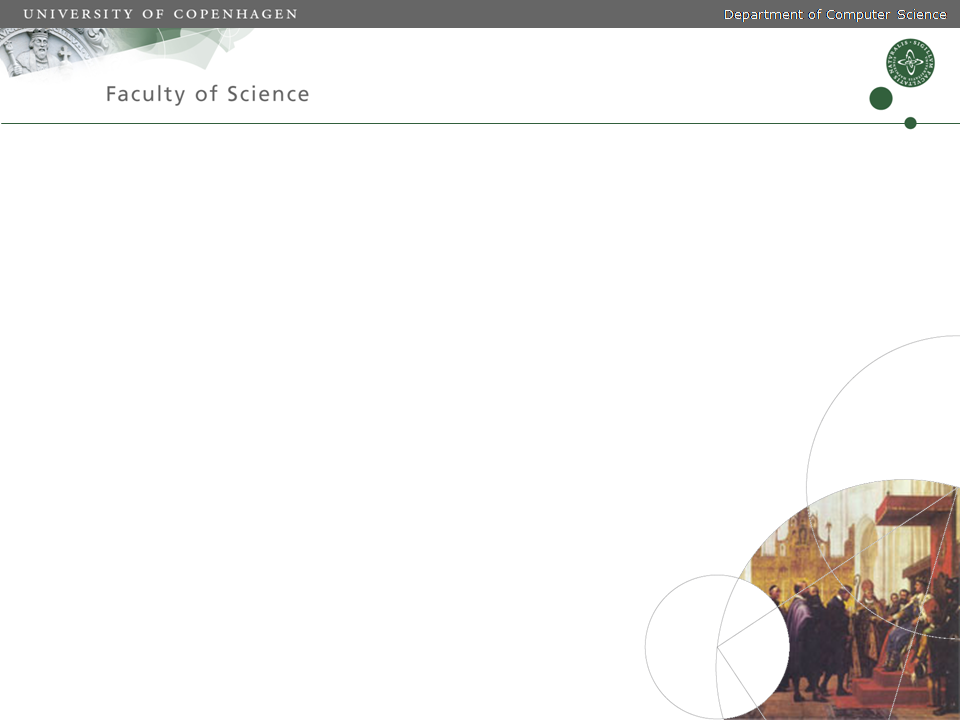
\includegraphics[width=\paperwidth,height=\paperheight]{front}}
%% {
%% \begin{frame}[plain]
%%   \titlepage
%% \end{frame}
%% }
%% }
\titleslide

\begin{frame}
\frametitle{Structure of a Compiler}

\begin{tabular}{ccc}
Program text&&\\
$\downarrow$ &&\\
\framebox{Lexical analysis} && Binary machine code\\
$\downarrow$ && $\uparrow$ \\
Symbol sequence && \textcolor{gray}{\framebox{Assembly and linking}} \\
$\downarrow$ && $\uparrow$ \\
\framebox{Syntax analysis} && Ditto with named registers\\
$\downarrow$ && $\uparrow$ \\
Syntax tree && \framebox{Register allocation} \\
$\downarrow$ && $\uparrow$ \\
\framebox{Typecheck} && Symbolic machine code\\
$\downarrow$ &&  $\uparrow$ \\
Syntax tree  && \framebox{Machine code generation} \\
$\downarrow$ && $\uparrow$ \\
\red{\framebox{Intermediate code generation}} &$\longrightarrow$ & \red{Intermediate code}
\end{tabular}

\end{frame}


\begin{frame}
	\tableofcontents

\end{frame}


\section{Why Intermediate Code?}


\begin{frame}
	\frametitle{Why Intermediate Code?}

\begin{itemize}
    \item Compilers for different platforms and languages can share parts.\bigskip

\begin{center}
\unitlength0.3em
\begin{picture}(100,20)
\put(0,0){\framebox(15,4){C++}}
\put(0,8){\framebox(15,4){Pascal}}
\put(0,16){\framebox(15,4){Fortran}}

\put(15,2){\vector(2,1){15}}
\put(15,10){\vector(1,0){15}}
\put(15,18){\vector(2,-1){15}}

\put(30,8){\framebox(22,4){Intermed.Code}}

\put(52,10){\vector(2,1){15}}
\put(52,10){\vector(1,0){15}}
\put(52,10){\vector(2,-1){15}}

\put(67,0){\framebox(15,4){X86}}
\put(67,8){\framebox(15,4){X86\_64}}
\put(67,16){\framebox(15,4){ARM}}

%\uncover<2->{
\qbezier(45,8)(55,0)(40,0)
\qbezier(40,0)(25,0)(35,8)
\put(35,8){\vector(1,1){0}}
%}
\end{picture}
\end{center}

\bigskip
 
    \item Machine-independent optimizations are possible.\bigskip
    \item Also enables interpretation ...\bigskip
\end{itemize}

\end{frame}



\subsection{Intermediate Language}

\begin{frame}
	\frametitle{Intermediate Language (\textsc{IL})}

\begin{itemize}

\item \emph{Machine Independent}: 
        no limit on register and memory, no machine-specific instructions.\bigskip

\item \emp{Mid-level(s)} between source and machine languages (\alert{tradeoff}):\\
                simpler constructs, easier to generate machine code.\bigskip

\item What features/constructs should \textsc{IL} support?\smallskip
    \begin{itemize}
        \item every translation loses information;\smallskip
        \item use the information before losing it!
    \end{itemize} \bigskip

\item How complex should \textsc{IL}'s instruction be?\smallskip
    \begin{itemize}
        \item complex: good for interpretation (amortizes instruction-decoding overhead),\smallskip
        \item simple: can more easily generate optimal machine code.\smallskip
    \end{itemize}

\end{itemize}
\end{frame}


\begin{frame}
	\frametitle{Intermediate Language (\textsc{IL})}

\begin{columns}

\column{0.42\textwidth}

\emp{Here:} 
	Low-level language, but keeping functions (procedures).
	
	Small instructions:
\begin{itemize}
\item \emph{3-address code}: one operation per expression
\pause
\item \emph{Memory} read/write (\cd{M}) (address is atom).
\pause
\item \emph{Jump} labels, \cd{GOTO} and 
	conditional jump (\cd{IF}).
\pause
\item \emph{Function} calls and returns
\end{itemize}


\column{0.62\textwidth}


{\footnotesize
\vspace*{-3ex}

%\hspace*{-2em}
%\begin{tabular}{p{0.8\textwidth}}
\[\begin{array}{lcl}
\mathit{Prg} & \rightarrow & \mathit{Fcts} \\
\mathit{Fcts}  & \rightarrow & \mathit{Fct~Fcts} \mid \mathit{Fct}\\
\mathit{Fct} & \rightarrow & \mathit{Hdr~Bd}\\
\mathit{Hdr} & \rightarrow & \mathbf{functionid}( \mathit{Args} ) \\
\mathit{Bd} & \rightarrow & [~\mathit{Instrs}~] \\[1ex]
\mathit{Instrs} & \rightarrow & \mathit{Instr~,~Instrs} \mid \mathit{Instr} \\
%
% 3-address code:
\mathit{Instr} & \rightarrow & 
%& & \mid 	
\mathbf{id} := \mathit{Atom}\mid % \\
%\mathit{Instr} & \rightarrow & 
% & & \mid 
\mathbf{id} := \mathbf{unop}~ \mathit{Atom} \\
%\mathit{Instr} & \rightarrow & 
& & \onslide<2->{\mid \mathbf{id} := \mathbf{id} ~ \mathbf{binop}~ \mathit{Atom}} \\
%\mathit{Instr} & \rightarrow & 
& & \onslide<3->{\mid \mathbf{id} := M[\mathit{Atom}] \mid % \\
%\mathit{Instr} & \rightarrow & 
	M[\mathit{Atom}]  := \mathbf{id}} \\
%\mathit{Instr} & \rightarrow & 
%\mathit{Instr} & \rightarrow & 
%\mathit{Instr} & \rightarrow & 
%\mathit{Instr} & \rightarrow & 
& & \onslide<4->{\mid \mathtt{LABEL}~\mathbf{label} \mid %\\
	\mathtt{GOTO}~ \mathbf{label} }\\
%\mathit{Instr} & \rightarrow &
& & \onslide<4->{\mid \mathtt{IF}~ \mathbf{id}~\mathbf{relop}~\mathit{Atom}}\\
& & \onslide<4->{\hspace*{2em}~\mathtt{THEN}~\mathbf{label}~\mathtt{ELSE}~\mathbf{label}} \\
& & \onslide<5->{\mid \mathbf{id} := \mathtt{CALL}~ \mathbf{functionid}( \mathit{Args} )}\\
& & \onslide<5->{\mid \mathtt{RETURN}~\mathbf{id} } \\
\mathit{Atom} & \rightarrow & \mathbf{id} \mid \mathbf{num} \\
\onslide<5->{\mathit{Args}} & \onslide<5->{\rightarrow} & \onslide<5->{\mathbf{id}~,~\mathit{Args} \mid \mathbf{id} }
\end{array}\]
%\end{tabular}
}


\end{columns}

\end{frame}


\subsection{To-Be-Translated Language}


\begin{frame}[fragile]
	\frametitle{The To-Be-Translated Language}
	
We shall translate a simple procedural language:
\begin{itemize}
\item Arithmetic expressions and function calls, boolean expressions,\smallskip
\item conditional branching (\cd{if}), \smallskip
\item two loops constructs (\cd{while} and \cd{repeat until}).\bigskip
\end{itemize}

\emph{Syntax-directed} translation:\smallskip
\begin{itemize}
\item In practice we work on the abstract syntax tree \textsc{AbSyn}\\
        (but here we use a generic grammar notation),\smallskip

\item Implement each \emph{syntactic category} via a \emp{translation function}:\\
    \emph{Arithmetic expressions, Boolean expressions, Statements.}


\item Code for subtrees is generated \emph{independent of context},\\
        (i.e., context is a parameter to the translation function)
\end{itemize}

\end{frame}


\section{Syntax-Directed Translation}

\subsection{Arithmetic Expressions}

\begin{frame}
	\tableofcontents[currentsubsection]
\end{frame}


\begin{frame}[fragile]
	\frametitle{Translating Arithmetic Expressions}

\begin{columns}
\column{0.6\textwidth}

\emph{Expressions in Source Language}
\begin{itemize}
\item Variables and number literals,
\item unary and binary operations,
	%(assume equivalent ones in intermediate code,
	%translation by \cd{trans\_op}),

\item function calls (with argument list).
\end{itemize}

\column{0.4\textwidth}

{\footnotesize

\renewcommand{\arraystretch}{0.75}
\[\begin{array}{lcl}
Exp & \rightarrow & {\bf num} \mid {\bf id}\\
%Exp & \rightarrow & {\bf id} \\
%Exp & \rightarrow & 
& & \mid {\bf unop}~Exp \\
%Exp & \rightarrow & 
& & \mid Exp~{\bf binop}~Exp \\
%Exp & \rightarrow &
& & \mid {\bf id}(Exps) \\
\\
Exps & \rightarrow & Exp \mid Exp~,~Exps
\end{array}\]

}
\end{columns}
\bigskip

\pause

Translation function:

\begin{colorcode}
\mymath{Trans\myindx{Exp}} :: (Exp, VTable, FTable, Location) -> [ICode]
\end{colorcode}

\begin{itemize}
\item Returns a list of intermediate code instructions \cd{[ICode]} that \ldots
\item \ldots upon execution, computes \cd{Exp}'s result in variable \cd{Location}.
\item \emph{Case analysis} on \cd{Exp}'s abstract syntax tree \textsc{AbSyn}.
\end{itemize}

\end{frame}

\begin{frame}[fragile, t]
	\frametitle{Symbol Tables and Helper Functions}

Translation function:

\begin{colorcode}
\mymath{Trans\myindx{Exp}} :: (Exp, VTable, FTable, Location) -> [ICode]
\end{colorcode}

\emph{Symbol Tables}
\begin{description}
\item[\emp{\em vtable}]: 
	variable names to intermediate code variables

\item[\emp{\em ftable}]: 
	function names to function labels (for \cd{call})
\end{description}

\bigskip

\emph{Helper Functions}
\begin{itemize}
\item \emp{lookup}: retrieve entry from a symbol table
\item \emp{getvalue}: retrieve value of source language literal
\item \emp{getname}: retrieve name of source language variable/operation
\item \emp{newvar}: make new intermediate code variable
\item \emp{newlabel}: make new label (for jumps in intermediate code)
\item \emp{trans\_op}: translates an operator name to the name in \textsc{IL}.
\end{itemize}

\end{frame}

\newcommand{\concat}{\mbox{\tt ~@~}}%\!\mbox{\tt +}}

\begin{frame}[fragile, t]
	\frametitle{Generating Code for an Expression}

%\begin{colorcode}
% \mymath{Trans\myindx{Exp}} :: (Exp, VTable, FTable, Location) -> [ICode]
%\end{colorcode}

{\footnotesize
\renewcommand{\arraystretch}{0.97}
%\begin{tabular}{|p{4cm}|l|l|}
\begin{tabular}{p{1.5cm}ll}
%\hline
\multicolumn{3}{l}{
    \emp{\mymath{Trans\myindx{Exp}}}\cd{ : (Exp, VTable, FTable, \green{Location}) -> [ICode]}}\\
%\multicolumn{3}{l}{\cd{trans\_exp} $ (exp,vtable,ftable,place)
% = \mbox{\tt case}~exp~\mbox{\tt of}$} \\

\multicolumn{3}{l}{\emp{\mymath{Trans\myindx{Exp}}} $ (exp,vtable,ftable,\green{place})
 = \mbox{\tt case}~exp~\mbox{\tt of}$} \\\hline

& {\bf num} & $v = getvalue({\bf num})$ \\
&        & $ [\green{place} := v]$ \\\hline

& {\bf id} & $x = lookup(vtable,getname({\bf id}))$ \\
&         & $ [\green{place} := x]$ \\\hline

&${\bf unop}~Exp_1$
        & $place_1 = newvar()$ \\
&        & $code_1 = \emp{Trans_{Exp}}(Exp_1,vtable,ftable,place_1)$ \\
&        & $op = \mbox{\tt trans\_op}(getname({\bf unop}))$ \\
&        & $code_1 \concat [\green{place} := op~place_1]$ \\\hline

&$Exp_1~{\bf binop}~Exp_2$
        & $place_1 = newvar()$ \\
&        & $place_2 = newvar()$ \\
&        & $code_1 = \emp{Trans_{Exp}}(Exp_1,vtable,ftable,place_1)$ \\
&        & $code_2 = \emp{Trans_{Exp}}(Exp_2,vtable,ftable,place_2)$ \\
&        & $op =     \mbox{\tt trans\_op}(getname({\bf binop}))$ \\
&        & $code_1 \concat code_2 \concat [\green{place} := place_1~op~place_2]$ \\\hline

%&${\bf id}(Exps)$
%        & $(code_1,[a_1,\ldots,a_n])$\\
%&        & $\hfill {} = \emp{Trans_{Exp}}(Exps,vtable,ftable)$ \\
%&        & $fname = lookup(ftable,getname({\bf id}))$ \\
%&        & $code_1 \concat [\green{place} := {\tt CALL}~fname(a_1,\ldots,a_n)]$ \\\hline
\end{tabular}
}

\end{frame}

\begin{frame}[fragile, t]
	\frametitle{Generating Code for a Function Call}


{\footnotesize
\renewcommand{\arraystretch}{0.97}
\begin{tabular}{p{1.5cm}ll}
\multicolumn{3}{l}{\emp{\mymath{Trans\myindx{Exp}}} $ (exp,vtable,ftable,\green{place})
 = \mbox{\tt case}~exp~\mbox{\tt of}$} \\\hline

&${\bf id}(Exps)$
        & $(code_1,[a_1,\ldots,a_n])~=~\red{Trans_{Exps}}(Exps,vtable,ftable)$ \\
&        & $fname = lookup(ftable,getname({\bf id}))$ \\
&        & $code_1 \concat [\green{place} := {\tt CALL}~fname(a_1,\ldots,a_n)]$ \\\hline
\end{tabular}
}

\bigskip

$\red{Trans_{Exps}}$ returns the code that evaluates the function's parameters,
and the list of new-intermediate variables (that store the result).

\bigskip

{\footnotesize

\renewcommand{\arraystretch}{0.97}
\begin{tabular}{p{1.5cm}ll}%\hline
\multicolumn{3}{l}{
	$\red{Trans_{Exps}}$ \cd{~:~(Exps, VTable, FTable) -> ([ICode], [\green{Location}]) }}\\
\multicolumn{3}{l}{$\red{Trans_{Exps}}(exps,vtable,ftable)
 = \mbox{\tt case}~exps~\mbox{\tt of}$} \\\hline

&$Exp$   & $place = newvar()$ \\
&        & $code_1 = \emp{Trans_{Exp}}(Exp,vtable,ftable,place)$ \\
&        & $(code_1,[\green{place}])$ \\\hline

&$Exp~,~Exps$
         & $place = newvar()$ \\
&        & $code_1 = \emp{Trans_{Exp}}(Exp,vtable,ftable,place)$ \\
&        & $(code_2,args) = \red{Trans_{Exps}}(Exps,vtable,ftable)$ \\
&        & $code_3 = code_1 \concat code_2$ \\
&        & $\green{args_1 = place :: args}$ \\
&        & $(code_3,\green{args_1})$ \\\hline

\end{tabular}
}

\end{frame}

\begin{frame}[fragile]
	\frametitle{Translation Example}

Assume the following symbol tables:
\begin{itemize}
\item \emph{vtable} $ = [ x \mapsto v0,\ y \mapsto v1,\ z \mapsto v2 ] $
\item \emph{ftable} $ = [ f \mapsto \_F\_1 ] $
\end{itemize}
Translation of \cd{Exp} with place = $ t0 $:

\begin{itemize}

\item \cd{Exp}=\cd{x-3}
\visible<2->{
\footnotesize
	\begin{minipage}{0.4\textwidth}
\renewcommand{\arraystretch}{0.9}
\[\begin{array}{l}
{\tt t1} := {\tt v0} \\
{\tt t2} := 3\\
{\tt t0} := {\tt t1} - {\tt t2} \\
\end{array}\]
	\end{minipage}
}

\pause \pause
\item \cd{Exp}=\cd{3+f(x-y,z)}
\visible<4->{
\footnotesize
\begin{minipage}{0.4\textwidth}
\renewcommand{\arraystretch}{0.9}
\[\begin{array}{l}
~~{\tt t1} := 3 \\
~~~~~~{\tt t4} := {\tt v0} \\
~~~~~~{\tt t5} := {\tt v1} \\
~~~~{\tt t3} := {\tt t4 - t5} \\
~~~~{\tt t6} := {\tt v2} \\
~~{\tt t2} := {\tt CALL~ \_F\_1(t3,t6)} \\
{\tt t0} := {\tt t1 + t2}
\end{array}\]
	\end{minipage}
}
\end{itemize}

\end{frame}

\subsection{Statements}

\begin{frame}
	\tableofcontents[currentsubsection]
\end{frame}

\begin{frame}[fragile]
	\frametitle{Translating Statements}

\begin{columns}
\column{0.5\textwidth}

\emph{Statements in Source Language}
\begin{itemize}
\item Sequence of statements
\item Assignment
\item Conditional Branching
\item Loops: \cd{while} and \cd{repeat}

	(simple conditions for now)
\end{itemize}

\column{0.55\textwidth}

{\footnotesize

\renewcommand{\arraystretch}{0.75}
\[\begin{array}{lcl}
Stat & \rightarrow & Stat~;~Stat \\
%Stat & \rightarrow & 
& & \mid {\bf id} := Exp \\
%Stat & \rightarrow & 
& & \mid {\tt if}~Cond~{\tt then}~\{~Stat~\} \\
%Stat & \rightarrow & 
& & \mid {\tt if}~Cond~{\tt then}~\{~Stat~\}~{\tt else}~\{~Stat~\} \\
%Stat & \rightarrow & 
& & \mid {\tt while}~Cond~{\tt do}~\{~Stat~\} \\
%Stat & \rightarrow & 
& & \mid {\tt repeat}~\{~Stat~\}~{\tt until}~Cond \\[1ex]
Cond & \rightarrow & Exp~ {\bf relop}~ Exp
\end{array}\]

}
\end{columns}
\smallskip

We assume relational operators translate directly (using \cd{trans\_op}).

\pause

\bigskip
Translation function:

\begin{colorcode}
\mymath{Trans\myindx{Stat}} :: (Stat, VTable, FTable) -> [ICode]
\end{colorcode}

\begin{itemize}
\item As before: syntax-directed, \emph{case analysis} on \cd{Stat}
\item Intermediate code instructions for statements
\end{itemize}

\end{frame}

\begin{frame}[fragile,t]
	\frametitle{Generating Code for Sequences, Assignments,\ldots}

\medskip

{ \footnotesize

\begin{tabular}{lll}
\multicolumn{3}{l}{
$\emp{Trans_{Stat}}$\cd{~:~(Stat, Vtable, Ftable) -> [ICode]}}\\
\multicolumn{3}{l}{
$\emp{Trans_{Stat}} (stat,vtable,ftable) = \mbox{\tt case}~stat~\mbox{\tt of}$} \\\hline

&$Stat_1~;~Stat_2$
        & $code_1 = \emp{Trans_{Stat}}(Stat_1,vtable,ftable)$ \\
&        & $code_2 = \emp{Trans_{Stat}}(Stat_2,vtable,ftable)$ \\
&        & $code_1 \concat code_2$ \\\hline

&${\bf id} := Exp$
        & $\green{place} = lookup(vtable,getname({\bf id}))$ \\
&        & $\red{Trans_{Exp}} (Exp,vtable,ftable,\green{place})$ \\\hline
&&\\
& \ldots  & (rest coming soon)\\
\end{tabular}
}

\begin{itemize}
\item Sequence of statements, sequence of code.
\item Symbol tables are inherited attributes.
\end{itemize}

\end{frame}

\begin{frame}[fragile,t]
	\frametitle{Generating Code for Conditional Jumps: Helper}

\begin{itemize}
\item Helper function for loops and branches

\item \emph{Evaluates} {\tt Cond}, i.e., a boolean expression, \\
	\emph{then jumps} to one of two labels, \emph{depending on result}

\end{itemize}

\bigskip

{\footnotesize
\renewcommand{\arraystretch}{0.9}
\begin{tabular}{lll}%\hline
\multicolumn{3}{l}{
$\emp{Trans_{Cond}}$ \cd{~:~(Cond, Label, Label, Vtable, Ftable) -> [ICode]}} \\
\multicolumn{3}{l}{$\emp{Trans_{Cond}} (cond,label_t,label_f,vtable,ftable) = \mbox{\tt case}~cond~\mbox{\tt of}$} \\\hline

&$Exp_1~{\bf relop}~Exp_2$
         & $t_1 = newvar()$ \\
&        & $t_2 = newvar()$ \\
&        & $code_1 = \red{Trans_{Exp}}(Exp_1,vtable,ftable,t_1)$ \\
&        & $code_2 = \red{Trans_{Exp}}(Exp_2,vtable,ftable,t_2)$ \\
&        & $op = \mbox{\tt trans\_op}(getname({\bf relop}))$ \\
&        & $code_1 \concat code_2 \concat [\emp{{\tt IF}~t_1\,op\,t_2~{\tt THEN}~label_t~{\tt ELSE}~label_f}]$\\[1ex]\hline
\end{tabular}
}

\bigskip

\begin{itemize}
\item Uses the \cd{IF} of the intermediate language
\item Expressions need to be evaluated before 

	(\emp{restricted \cd{IF}: only variables and atoms can be used})
\end{itemize}
\end{frame}

\begin{frame}[fragile,t]
	\frametitle{Generating Code for If-Statements}

\begin{itemize}
\item Generate \emph{new labels} for branches and following code

\item Translate \cd{If} statement to a \emph{conditional jump}

\end{itemize}
\pause

\bigskip

{\footnotesize
\renewcommand{\arraystretch}{0.9}
\begin{tabular}{lll}%\hline
%\multicolumn{3}{l}{
%\cd{trans\_stat : (Stat, Vtable, Ftable) -> [ICode]}} \\
\multicolumn{3}{l}{$\emp{Trans_{Stat}}(stat,vtable,ftable)
 = \mbox{\tt case}~stat~\mbox{\tt of}$} \\\hline

&${\tt if}~Cond$
        & $\green{label_t} = newlabel()$ \\
&${\tt then}~Stat_1$
        & $\red{label_f} = newlabel()$ \\
&        & $code_1 = Trans_{Cond}(Cond,\green{label_t},\red{label_f},vtable,ftable)$ \\
&        & $code_2 = \emp{Trans_{Stat}}(Stat_1,vtable,ftable)$ \\
&        & $code_1 \concat [{\tt LABEL}~\green{label_t}] 
	\concat code_2 \concat [{\tt LABEL}~\red{label_f}]$ \\\hline
%\pause 
&${\tt if}~Cond$
        & $\green{label_t} = newlabel()$ \\
&${\tt then}~Stat_1$
        & $\red{label_f} = newlabel()$ \\
&${\tt else}~Stat_2$
        & $\blue{label_e} = newlabel()$ \\
&        & $code_1 = Trans_{Cond}(Cond,\green{label_t},\red{label_f},vtable,ftable)$ \\
&        & $code_2 = \emp{Trans_{Stat}}(Stat_1,vtable,ftable)$ \\
&        & $code_3 = \emp{Trans_{Stat}}(Stat_2,vtable,ftable)$ \\
&        & $code_1 \concat [{\tt LABEL}~\green{label_t}] \concat code_2 \concat [\blue{{\tt GOTO}~label_e}] $\\
&        & $~~~~~~~\concat [{\tt LABEL}~\red{label_f}] \concat code_3 \concat [{\tt LABEL}~\blue{label_e}]$ \\\hline

\end{tabular}
}
%
%\begin{itemize}
%
%\item \emph{Without \cd{else}:} jump to \cd{then} branch or to following code
%
%\item \emph{With \cd{else}:} jump to \cd{then} branch or to \cd{else} branch,
%	and insert another jump instruction at end of \cd{then} branch.
%
%\end{itemize}
%
\end{frame}

\begin{frame}[fragile]
	\frametitle{Generating Code for Loops}

\begin{itemize}
\item \cd{repeat-until} loop is the easy case:

	Execute body, check condition, jump back if false.

\item \cd{while} loop needs check before body, one extra label needed.
\end{itemize}
\pause
{\footnotesize
\renewcommand{\arraystretch}{0.9}
\begin{tabular}{lll}%\hline
%\multicolumn{3}{l}{
%\cd{trans\_stat : (Stat, Vtable, Ftable) -> [ICode]}} \\
\multicolumn{3}{l}{$ \emp{Trans_{Stat}}(stat,vtable,ftable)
 = \mbox{\tt case}~stat~\mbox{\tt of}$} \\\hline

&${\tt repeat}~Stat$
        & $\red{label_f} = newlabel()$ \\
&${\tt until}~Cond$
        & $\green{label_t} = newlabel()$ \\
&        & $code_1 = \emp{Trans_{Stat}}(Stat,vtable,ftable)$ \\
&        & $code_2 = Trans_{Cond}(Cond,\green{label_t},\red{label_f},vtable,ftable)$ \\
&        & $[{\tt LABEL}~\red{label_f}] \concat code_1 
		\concat code_2 \concat [{\tt LABEL}~\green{label_t}]$ \\\hline

&${\tt while}~Cond$
        & $\blue{label_s} = newlabel()$ \\
&${\tt do}~Stat$
        & $\green{label_t} = newlabel()$ \\
&        & $\red{label_f} = newlabel()$ \\
&        & $code_1 = Trans_{Cond}(Cond,\green{label_t},\red{label_f},vtable,ftable)$ \\
&        & $code_2 = \emp{Trans_{Stat}}(Stat,vtable,ftable)$ \\
&        & $ [{\tt LABEL}~\blue{label_s}] \concat code_1 $ \\
&        & $ \concat [{\tt LABEL}~\green{label_t}] \concat code_2 \concat [\blue{{\tt GOTO}~label_s}] $\\
&        & $~~~~~~~\concat [{\tt LABEL}~\red{label_f}] $\\\hline
\end{tabular}
}

\end{frame}

\begin{frame}[fragile,t]
	\frametitle{Translation Example}

\begin{itemize}
\item Symbol table \emp{vtable}: $ [ x \mapsto v_0,\ y\mapsto v_1,\ z \mapsto v_2] $

\item Symbol table \emp{ftable}: $ [ {\tt getInt} \mapsto {\tt libIO\_getInt} ] $
\end{itemize}

\vspace*{-3ex}
\begin{columns}

\column[t]{0.35\textwidth}
\begin{colorcode}[frame=lines]
\red{x := 3;}
\orange{y := getInt();}
z := 1;
\blue{while y > 0}
    y := y - 1;
\green{    z := z * x}
\end{colorcode}

\column[t]{0.5\textwidth}
\medskip

{\raggedright \footnotesize
\visible<2->{
\texttt{\red{v\_0 := 3}}\\
\texttt{\orange{v\_1 := CALL libIO\_getInt()}}\\
\texttt{{v\_2 := 1}}\\
\visible<3->{
\texttt{\blue{~LABEL l\_s}}\\
\texttt{\blue{~~t\_1 := v\_1}}\\
\texttt{\blue{~~t\_2 := 0}}\\
\texttt{\blue{~~IF t\_1 $ > $ t\_2 THEN l\_t else l\_f}}\\
\texttt{\blue{~~LABEL l\_t}}\\
\visible<4->{
\texttt{~~~t\_3 := v\_1}\\
\texttt{~~~t\_4 := 1}\\
\texttt{~~~v\_1 := t\_3 - t\_4}\\
\visible<5->{
\texttt{\green{~~~t\_5 := v\_2}}\\
\texttt{\green{~~~t\_6 := v\_0}}\\
\texttt{\green{~~~v\_2 := t\_5 * t\_6}}\\
}}
\texttt{\blue{~~GOTO l\_s}}\\
\texttt{\blue{~LABEL l\_f}}\\
}}}

\end{columns}

\end{frame}

\subsection{Boolean Expressions, Sequential Evaluation}

\begin{frame}
	\tableofcontents[currentsubsection]
\end{frame}


\begin{frame}[fragile]
	\frametitle{More Complex Conditions, Boolean Expressions}


\begin{columns}
\column{0.53\textwidth}

\emph{Boolean Expressions as Conditions}
\begin{itemize}
%\item Constants \textbf{true} and \textbf{false}
\item Arithmetic expressions used as Boolean
\item Logical operators (not, and, or)
\item Boolean expressions used in arithmetics

\end{itemize}

\column{0.45\textwidth}

{\footnotesize

\renewcommand{\arraystretch}{0.9}
\[\begin{array}{lcl}
Cond & \rightarrow & Exp~\mbox{\bf relop}~ Exp\\
%& & \mid \mbox{\tt true} \mid \mbox{\tt false}\\
& & \mid Exp\\
& & \mid \mbox{\bf not}~Cond\\
& & \mid Cond~\mbox{\bf and}~Cond\\
& & \mid Cond~\mbox{\bf or}~Cond\\[1ex]
Exp & \rightarrow & \ldots \mid Cond\\
\end{array}\]

}
\end{columns}

\bigskip
\bigskip

\pause
We extend the translation functions $Trans_{Exp}$ and $Trans_{Cond}$:

\begin{itemize}
%\item \emph{Boolean expressions} are used as conditions.
\item \emph{Interpret numeric values} as Boolean expressions: 

	0 is \textbf{false}, all other values \textbf{true}.
\item Likewise: \emph{truth values as arithmetic expressions}

\end{itemize}

\end{frame}


\begin{frame}[fragile]
	\frametitle{Numbers and Boolean Values, Negation}

\emp{Expressions as Boolean values, negation:}
\smallskip

{\footnotesize
\renewcommand{\arraystretch}{0.9}
\begin{tabular}{lll}%\hline
\multicolumn{3}{l}{
$\red{Trans_{Cond}}$\cd{~:~(Cond, Label, Label, Vtable, Ftable) -> [ICode]}} \\
\multicolumn{3}{l}{$\red{Trans_{Cond}}(cond,label_t,label_f,vtable,ftable)
 = \mbox{\tt case}~cond~\mbox{\tt of}$} \\
& \ldots &\\\hline
&$Exp$
        & $t = newvar()$ \\
&        & $code = \emp{Trans_{Exp}}(Exp,vtable,ftable,t)$ \\
&        & $code \concat [{\tt IF}~t \neq 0~{\tt THEN}~label_t~{\tt ELSE}~label_f]$\\[1ex]\hline
&$ \mbox{\bf not} Cond$
	    & $\red{Trans_{Cond}}(Cond,label_f, label_t, vtable,ftable)$ \\[1ex]\hline
& \ldots &
\end{tabular}
}

\bigskip
\uncover<2->{
\emp{Conversion of Boolean values to numbers (by jumps):}
\smallskip

{\footnotesize
\renewcommand{\arraystretch}{0.9}
\begin{tabular}{lll}%\hline
\multicolumn{3}{l}{
$\emp{Trans_{Exp}}$\cd{~:~(Exp, Label, Label, Vtable, Ftable) -> [ICode]}} \\
\multicolumn{3}{l}{$\emp{Trans_{Exp}}(exp,vtable,ftable, place)
 = \mbox{\tt case}~exp~\mbox{\tt of}$} \\
& \ldots &\\\hline
& $Cond$
	    & $label_1 = newlabel()$ \\
&        & $label_2 = newlabel()$ \\
&        & $t = newvar()$ \\
&        & $code = \red{Trans_{Cond}}(Cond,label_1,label_2,vtable,ftable)$\\
&        & $[t := 0] \concat code \concat [{\tt LABEL}~label_1,~t := 1]
			\concat [{\tt LABEL}~label_2,~place := t]$\\\hline
\end{tabular}
}
}
\end{frame}



\begin{frame}[fragile,t]
    \frametitle{Fasto Implementation for Conditionals/Comparisons}

\begin{block}{Fasto Implementation}
\begin{colorcode}[fontsize=\scriptsize]
fun compileExp e vtable place = case e of
      ...
    | Fasto.If (e1,e2,e3,pos) =>
        let val thenLab="..." val elseLab="..." val endLab="..."
            val code1 = compileCond e1 vtable thenLab elseLab
            val code2 = compileExp  e2 vtable place
            val code3 = compileExp  e3 vtable place
        in code1 @ [Mips.LABEL thenLab] @ code2 @ [Mips.J endLab    ] @
                   [Mips.LABEL elseLab] @ code3 @ [Mips.LABEL endLab] 
        end

and compileCond c vtable tlab flab = case c of
      Fasto.Equal (e1,e2,pos) =>
        let val t1 = "..."
            val t2 = "..."
            val code1 = compileExp e1 vtable t1
            val code2 = compileExp e2 vtable t2
        in code1 @ code2 @ [Mips.BEQ (t1,t2,tlab), Mips.J flab] 
        end
\end{colorcode} 
\end{block}

\end{frame}


\begin{frame}[fragile]
	\frametitle{Sequential Evaluation of Conditions}

\begin{colorcode}[fontsize=\scriptsize]
Moscow ML version 2.01 (January 2004)
Enter `quit();' to quit.
- fun f l = if (hd l = 1) then "one" else "not one";
> val f = fn : int list -> string
- f [];
! Uncaught exception: 
! Empty
\end{colorcode}
\pause

In most languages, 
logical operators are \emp{evaluated sequentially}.

\begin{itemize}
\item If $ B_1 = \mathit{false}$, do not evaluate $ B_2 $ in $ B_1 \&\& B_2 $ 
	(anyway \textit{false}).
\item If $ B_1 = \mathit{true}$, do not evaluate $ B_2 $ in $ B_1 || B_2 $
	(anyway \textit{true}).
\end{itemize}
\pause
\begin{colorcode}[fontsize=\scriptsize]
- fun g l = if not (null l) \alert{andalso} (hd l = 1) then "one" else "not one";
> val g = fn : int list -> string
- g [];
> val it = "not one" : string
\end{colorcode}

\end{frame}

\begin{frame}[fragile]
	\frametitle{Sequential Evaluation by ``Jumping Code''}

{\footnotesize
\renewcommand{\arraystretch}{0.9}
\begin{tabular}{lll}%\hline
\multicolumn{3}{l}{
$\emp{Trans_{Cond}}$\cd{~:~(Cond, Label, Label, Vtable, Ftable) -> [ICode]}} \\
\multicolumn{3}{l}{$\emp{Trans_{Cond}}(cond,\green{label_t},\red{label_f},vtable,ftable)
 = \mbox{\tt case}~cond~\mbox{\tt of}$} \\%\hline
& \ldots &\\\hline
&$Cond_1$
        & $\blue{label_{next}} = newlabel()$ \\
&$~~\mbox{\bf and}$
        & $code_1{=}\emp{Trans_{Cond}}(Cond_1,\blue{label_{next}},\red{label_f},vtable,ftable)$ \\
&$~~~~Cond_2$
        & $code_2{=}\emp{Trans_{Cond}}(Cond_2,\green{label_t},\red{label_f},vtable,ftable)$ \\
&        & $code_1\concat[{\tt LABEL}~\blue{label_{next}}]\concat code_2$\\[1ex]\hline

&$Cond_1$
        & $\blue{label_{next}} = newlabel()$ \\
&$~~\mbox{\bf or}$
        & $code_1{=}\emp{Trans_{Cond}}(Cond_1,\green{label_t},\blue{label_{next}},vtable,ftable)$ \\
&$~~~~Cond_2$
        & $code_2{=}\emp{Trans_{Cond}}(Cond_2,\green{label_t},\red{label_f},vtable,ftable)$ \\
&        & $code_1\concat[{\tt LABEL}~\blue{label_{next}}]\concat code_2$\\[1ex]\hline

\end{tabular}
}

\pause
\bigskip

\begin{itemize}
\item Note: No logical operations in intermediate language!

	Logics of \textbf{and} and \textbf{or} encoded by jumps.
\pause
\item \emph{Alternative}: Logical operators in intermediate language

{\footnotesize \centering $ Cond \Rightarrow Exp \Rightarrow Exp ~{\bf binop}~ Exp $\\}

Translated as an arithmetic operation. \pause \emp{Evaluates both sides!}

\end{itemize}

\end{frame}

\section{Translating More Complex Structures}

\begin{frame}[fragile]
	\tableofcontents[currentsection]

\end{frame}


\subsection{More Control Structures}

\begin{frame}[fragile,t]
	\frametitle{More Control Structures}

\begin{itemize}
\item \emph{Control structures} determine \emph{control flow}: which instruction to execute next

\item A \textbf{while}-loop is enough
\pause \ldots but \ldots
%\item 
languages usually offer more.

%\begin{itemize}
\item \emph{Explicit jumps}: 
{\footnotesize $ \begin{array}[t]{lll} 
Stat &\rightarrow &{\bf label:}\\
& &\mid {\bf goto}~{\bf label} 
\end{array}$
}

	Necessary instructions are in the intermediate language. 
	
	Needs to build symbol table of labels.

\pause
\item \emph{Case/Switch}:
{\footnotesize 
$ \begin{array}[t]{lll} 
Stat & \rightarrow &{\bf case}~Exp ~{\bf of}~[~Alts~]\\
Alts & \rightarrow & {\bf num:}~Stat \mid {\bf num:}~Stat ,~Alts
\end{array}$
}

	When exited after each case: chain of \cd{if-then-else}

	When ``falling through'' (e.g., in C): \cd{if-then-else} and \cd{goto}.
\pause
\item \emph{Break and Continue}:
{\footnotesize 
$ \begin{array}{lll} 
Stat & \rightarrow &{\bf break} \mid {\bf continue}
\end{array}$
}

	(\cd{break}: jump behind loop, \cd{continue}: jump to end of loop body).

	Needs two jump target labels used only inside loop bodies
	(parameters to translation function $Trans_{Stat}$)

\visible<5->{\vspace*{-5.9cm}
\hspace*{5cm}\rotatebox{5}{\red{\framebox{\small \bf \ldots considered harmful} {\tiny (Dijkstra 1968)}}}
}
\end{itemize}

%\end{itemize}

\end{frame}

\subsection{Arrays and Other Structured Data}

\begin{frame}
	\tableofcontents[currentsubsection]
\end{frame}


\begin{frame}[fragile,t]
	\frametitle{Translating Arrays (of {\tt int} elements)}

\begin{columns}
\column{0.6\textwidth}

\emph{Extending the Source Language}
\medskip

\begin{itemize}
\item Array elements used as an expression
\item Assignment to an array element
\item Array elements accessed by an index (expression)
\end{itemize}

\column{0.4\textwidth}

{\footnotesize

\renewcommand{\arraystretch}{1.1}
\[\begin{array}{lcl}
Exp & \rightarrow & \ldots \mid Idx\\
Stat & \rightarrow & \ldots \mid Idx ~:=~ Exp \\
Idx & \rightarrow & {\bf id}[~Exp~]\\
\end{array}\]

}
\end{columns}

\bigskip

\pause

Again we \emp{extend $Trans_{Exp}$ and $Trans_{Stat}$}.

\begin{itemize}

\item Arrays stored in \emph{pre-allocated memory area}, 
	generated code will \emph{use memory access instructions}.

\item Static (compile-time) or dynamic (run-time) allocation possible.

%\item Symbol table contains \emph{base address of array}.
%
%\item \emph{New translation function} \cd{trans\_idx}: compute address from index.
%
%	Elements are \cd{int} here, so 4 bytes per element for address.
%
\end{itemize}

\end{frame}

\begin{frame}[t]
	\frametitle{Generating Code for Address Calculation}

\begin{itemize}

\item \red{$vtable$} contains the \red{base address of the array}.

\item Elements are \texttt{int} here, so $4$ bytes per element for address.

\end{itemize}

\bigskip
{\footnotesize 
\begin{tabular}{lll}
\multicolumn{3}{l}{$\emp{Trans_{Idx}}(\mathit{index},\mathit{vtable},\mathit{ftable})
 = \mathtt{case}~\mathit{index}~\mathtt{of}$} \\\hline

&$\mathbf{id} [ \mathit{Exp} ]$
        & $\mathit{\red{base}} = \mathit{lookup}(\red{\mathit{vtable}},\mathit{getname}(\mathbf{id}))$ \\
&        & $\blue{addr} = \mathit{newvar}()$ \\
&        & $\mathit{code}_1 = \emph{Trans_{Exp}} (\mathit{Exp},\mathit{vtable},\mathit{ftable},\blue{addr})$ \\
&        & $\mathit{code}_2 = \mathit{code}_1 \concat [\blue{addr := addr} \red{* 4}, 
        	                                          \blue{addr := addr + }\mathit{\red{base}}]$ \\
&        & $(\emp{\mathit{code}_2},\blue{addr})$ \\\hline
\end{tabular}
}
\bigskip 

Returns: 
\begin{itemize}

\item \emp{Code to calculate the absolute address} \ldots
\item of the array element \emp{in memory} (corresponding to \texttt{index}), \ldots

\item \ldots and a new variable (\blue{\it addr}) where it will be stored.

\end{itemize}

\end{frame}

\begin{frame}[t]
	\frametitle{Generating Code for Array Access}

Address-calculation code: in expression and statement translation.

\bigskip

\begin{itemize}
\item \emph{Read access} inside expressions:

\medskip
{\footnotesize 
\begin{tabular}{lll}
\multicolumn{3}{l}{$Trans_{Exp}(\mathit{exp},\mathit{vtable},\mathit{ftable},\mathit{place})
 = \mathtt{case}~\mathit{exp}~\mathtt{of}$} \\
& \ldots &\\\hline
& $\mathit{Idx}$
        & $(\blue{\mathit{code}_1},\mathit{\blue{address}}) = Trans_{Idx} (\mathit{Idx},\mathit{vtable},\mathit{ftable})$ \\
&       & $\blue{\mathit{code}_1} \concat [\mathit{place} := M[\mathit{\blue{address}}]]$ \\\hline
\end{tabular}
}

\bigskip
\item \emph{Write access} in assignments:

\medskip
{\footnotesize 
\begin{tabular}{lll}
\multicolumn{3}{l}{$Trans_{Stat}(\mathit{stat},\mathit{vtable},\mathit{ftable})
 = \mathtt{case}~\mathit{stat}~\mathtt{of}$} \\
& \ldots &\\\hline
& $\mathit{Idx} := \mathit{Exp}$
        & $(\blue{\mathit{code}_1},\mathit{\blue{address}}) \,{=}\, Trans_{Idx}(\mathit{Index},\mathit{vtable},\mathit{ftable})$ \\
&        & $t = \mathit{newvar}()$ \\
&        & $\mathit{code}_2 = Trans_{Exp}(\mathit{Exp},\mathit{vtable},\mathit{ftable},t)$ \\
&        & $\blue{\mathit{code}_1} \concat \mathit{code}_2 \concat [M[\mathit{\blue{address}}] := t]$ \\\hline
\end{tabular}
}

\end{itemize}

\end{frame}
\begin{frame}[fragile,t]
	\frametitle{Multi-Dimensional Arrays}

\begin{columns}
\column{0.6\textwidth}

\emph{Arrays in Multiple Dimensions}
\medskip

\begin{itemize}
\item Only a small change to previous grammar:
	\textit{Idx} can now be \emp{recursive}.
\item Needs to be mapped to an address in one dimension.
\end{itemize}

\column{0.4\textwidth}

{\footnotesize

\renewcommand{\arraystretch}{1.1}
\[\begin{array}{lcl}
Exp & \rightarrow & \ldots \mid Idx\\
Stat & \rightarrow & \ldots \mid Idx ~:=~ Exp \\
Idx & \rightarrow & {\bf id}[Exp] \red{~\mid Idx[Exp]}\\
\end{array}\]

}
\end{columns}

\pause

\bigskip
\bigskip
\begin{itemize}

\item Arrays stored in \emph{row-major} or \emph{column-major} order.
\begin{minipage}{1mm}{\visible<2->{\vspace*{-1cm}~~~~~~~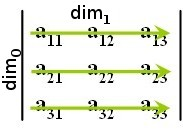
\includegraphics[b,height=1.5cm]{Figures/matrix_rows}}\vspace*{-1.5cm}}\end{minipage}

	\emp{Standard: row-major},
	index of \cd{a[k][l]} is $ k\cdot dim_1 + l$

	(Index of \cd{b[k][l][m]} is $ k\cdot dim_1 \cdot dim_2 + l \cdot dim_2 + m $)\smallskip
	
\pause

\item Address calculation \emph{need to know sizes} in each dimension.\\
    \emp{Symbol table: base address and list of array-dimension sizes.}\smallskip
%	(stored in symbol table with base address).

\item Need to change $Trans_{Idx}$, i.e., add recursive index calculation.

\end{itemize}

\end{frame}

\begin{frame}[fragile,t]
	\frametitle{Address Calculation in Multiple Dimensions}

{\footnotesize 
\begin{tabular}{lll}
\multicolumn{3}{l}{$Trans_{Idx}(\mathit{index},\mathit{vtable},\mathit{ftable}) = $}\\
\hline
&        & $(\mathit{code}_1, t, \mathit{base}, []) = \red{Calc_{Idx}} (\mathit{index},\mathit{vtable},\mathit{ftable})$ \\
&        & $\mathit{code}_2 = \mathit{code}_1 \concat [t := t*4, t := t+\mathit{base}]$ \\
&        & $(\mathit{code}_2,t)$ \\\hline
& &\\[2ex]
\end{tabular}
}

\pause

\emph{Recursive index calculation}, multiplies with dimension at each step.

\bigskip

{\footnotesize 
\begin{tabular}{lll}
\multicolumn{3}{l}{$\red{Calc_{Idx}}(\mathit{index},\mathit{vtable},\mathit{ftable})
 = \mathtt{case}~\mathit{index}~\mathtt{of}$} \\\hline

&$\mathbf{id} [ \mathit{Exp} ]$
        & $ (\mathit{base}, \mathit{dims})  = 
        	     \mathit{lookup}(\mathit{vtable},\mathit{getname}(\mathbf{id}))$ \\
&        & $\blue{addr} = \mathit{newvar}()$ \\
&        & $\mathit{code} = Trans_{Exp} (\mathit{Exp},\mathit{vtable},\mathit{ftable},\blue{addr})$ \\
&        & $(\mathit{code},\blue{addr}, \mathit{base}, \mathit{tail(dims)})$ \\\hline
&$\mathit{Index} [ \mathit{Exp} ]$
        & $(\mathit{code}_1, \blue{addr},\mathit{base},\mathit{dims}) = \red{Calc_{Idx}}(\mathit{Index},\mathit{vtable},\mathit{ftable})$ \\
&        & $\mathit{\green{d}} = \mathit{head}(\mathit{dims})$\\
&        & $\orange{t} = \mathit{newvar}()$ \\
&        & $\mathit{code}_2 = Trans_{Exp}(\mathit{Exp},\mathit{vtable},\mathit{ftable},\orange{t})$ \\
&        & $\mathit{code}_3 = \mathit{code}_1 \concat \mathit{code}_2 \concat [\blue{addr} := \blue{addr} * \mathit{\green{d}}, \blue{addr} := \blue{addr}+\orange{t} ]$ \\
&        & $(\mathit{code}_3,\blue{addr}, \mathit{base},\mathit{tail}(\mathit{dims}))$ \\\hline
\end{tabular}
}

\end{frame}

\subsection{Role of Declarations in the Translation}

\begin{frame}
	\tableofcontents[currentsubsection]
\end{frame}


\begin{frame}[fragile]
	\frametitle{Declarations in the Translation}

\emph{Declarations are necessary}

\begin{itemize}
\item to allocate space for arrays,
\item to compute addresses for multi-dimensional arrays,
\item \ldots and when the language allows \emph{local declarations (scope)}.
\end{itemize}

\pause

\begin{columns}
\column{0.6\textwidth}

\emph{Declarations and scope}
\begin{itemize}
\item Statements following a declarations can see declared data.
\item Declaration of variables and arrays
\item Here: Constant size, one dimension
\end{itemize}

\column{0.4\textwidth}

{\footnotesize

\renewcommand{\arraystretch}{0.9}
\[\begin{array}{lcl}
Stat & \rightarrow & Decl;~Stat\\
Decl & \rightarrow & {\tt int}~\mathbf{id}\\
& & \mid {\tt int}~\mathbf{id}[\mathbf{num}]\\
\end{array}\]
}
\end{columns}

\bigskip
Function $Trans_{Decl}$\cd{~:~(Decl, VTable) -> ([ICode], VTable)} 

\begin{itemize}
\item translates declarations to code and new symbol table.
\end{itemize}

\end{frame}

\begin{frame}
	\frametitle{Translating Declarations to Scope and Allocation}

Code with local scope (extended symbol table):
\medskip

{\footnotesize
\begin{tabular}{lll}
\multicolumn{3}{l}{$ Trans_{Stat}(\mathit{stat},\mathit{vtable},\mathit{ftable})
 = \mathtt{case}~\mathit{stat}~\mathtt{of}$} \\\hline

&$\mathit{Decl}~;~\mathit{Stat}_1$
        & $(\blue{\mathit{code}_1},\blue{\mathit{vtable}_1}) = \red{Trans_{Decl}}(\mathit{Decl},\mathit{vtable})$ \\
&        & $\mathit{code}_2 = Trans_{Stat}(\mathit{Stat}_1,\blue{\mathit{vtable}_1},\mathit{ftable})$ \\
&        & $\blue{\mathit{code}_1} \concat \mathit{code}_2$ \\\hline
\end{tabular}
}
\bigskip

\pause
Building the symbol table and allocating:
\medskip

{\footnotesize
\begin{tabular}{lll}
\multicolumn{3}{l}{$\red{Trans_{Decl}}$\cd{~:~(Decl, VTable) -> ([ICode], VTable )}}\\
\multicolumn{3}{l}{$\red{Trans_{Decl}}(\mathit{decl},\mathit{vtable})
 = \mathtt{case}~\mathit{decl}~\mathtt{of}$} \\\hline

&$\mathtt{int}~\mathbf{id}$
        & $t_1 = \mathit{newvar}()$ \\
&        & $\mathit{vtable}_1 = \mathit{bind}(\mathit{vtable}, \mathit{getname}(\mathbf{id}), t_1)$ \\
&        & $([],\:\mathit{vtable}_1)$ \\\hline
&$\mathtt{int}~\mathbf{id}{[}\mathbf{num}{]}$
        & $t_1 = \mathit{newvar}()$ \\
&        & $\mathit{vtable}_1 = \mathit{bind}(\mathit{vtable}, \mathit{getname}(\mathbf{id}), t_1)$ \\
&        & $([t_1 := HP,\, HP := HP + (4*\mathit{getvalue}(\mathbf{num}))],\:\mathit{vtable}_1)$ \\\hline
\end{tabular}

\bigskip

\ldots where \cd{HP} is the heap pointer, indicating the first free space in a managed heap at 
runtime; used for dynamic allocation.

}
\end{frame}

\begin{frame}
	\frametitle{Other Structures that Require Special Treatment}

\begin{itemize}
\item \emph{Floating-Point} values:

	Often stored in \emp{different registers}\\
	Always require \emp{different machine operations} 
	
	\emp{Symbol table needs type information} when creating variables in intermediate code.
	
\pause
\item \emph{Strings}

	Sometimes just arrays of (1-byte) \cd{char} type, but \emp{variable length}.

	In modern languages/implementations, elements can be 
	\cd{char} or \cd{unicode} (UTF-8 and UTF-16 \emph{variable size}!)
 
	Usually \emp{handled by library functions}.

\pause
\item \emph{Records} and \emph{Unions}

	Linear in memory. Field \emph{types and sizes} can be \emph{different}.

	\emp{Field selector} known at compile time: \emp{compute offset} from base.
\end{itemize}

\end{frame}


\begin{frame}
\frametitle{Structure of a Compiler}

\begin{tabular}{ccc}
Program text&&\\
$\downarrow$ &&\\
\framebox{Lexical analysis} && Binary machine code\\
$\downarrow$ && $\uparrow$ \\
Symbol sequence && \textcolor{gray}{\framebox{Assembly and linking}} \\
$\downarrow$ && $\uparrow$ \\
\framebox{Syntax analysis} && Ditto with named registers\\
$\downarrow$ && $\uparrow$ \\
Syntax tree && \framebox{Register allocation} \\
$\downarrow$ && $\uparrow$ \\
\framebox{Typecheck} && Symbolic machine code\\
$\downarrow$ &&  $\uparrow$ \\
Syntax tree  && \framebox{Machine code generation} \\
$\downarrow$ && $\uparrow$ \\
\red{\framebox{Intermediate code generation}} &$\longrightarrow$ & \red{Intermediate code}
\end{tabular}

\end{frame}


%\begin{frame}\huge \centering So far for today\\ \end{frame} 


\end{document}
